\begin{figure}
	\centering
	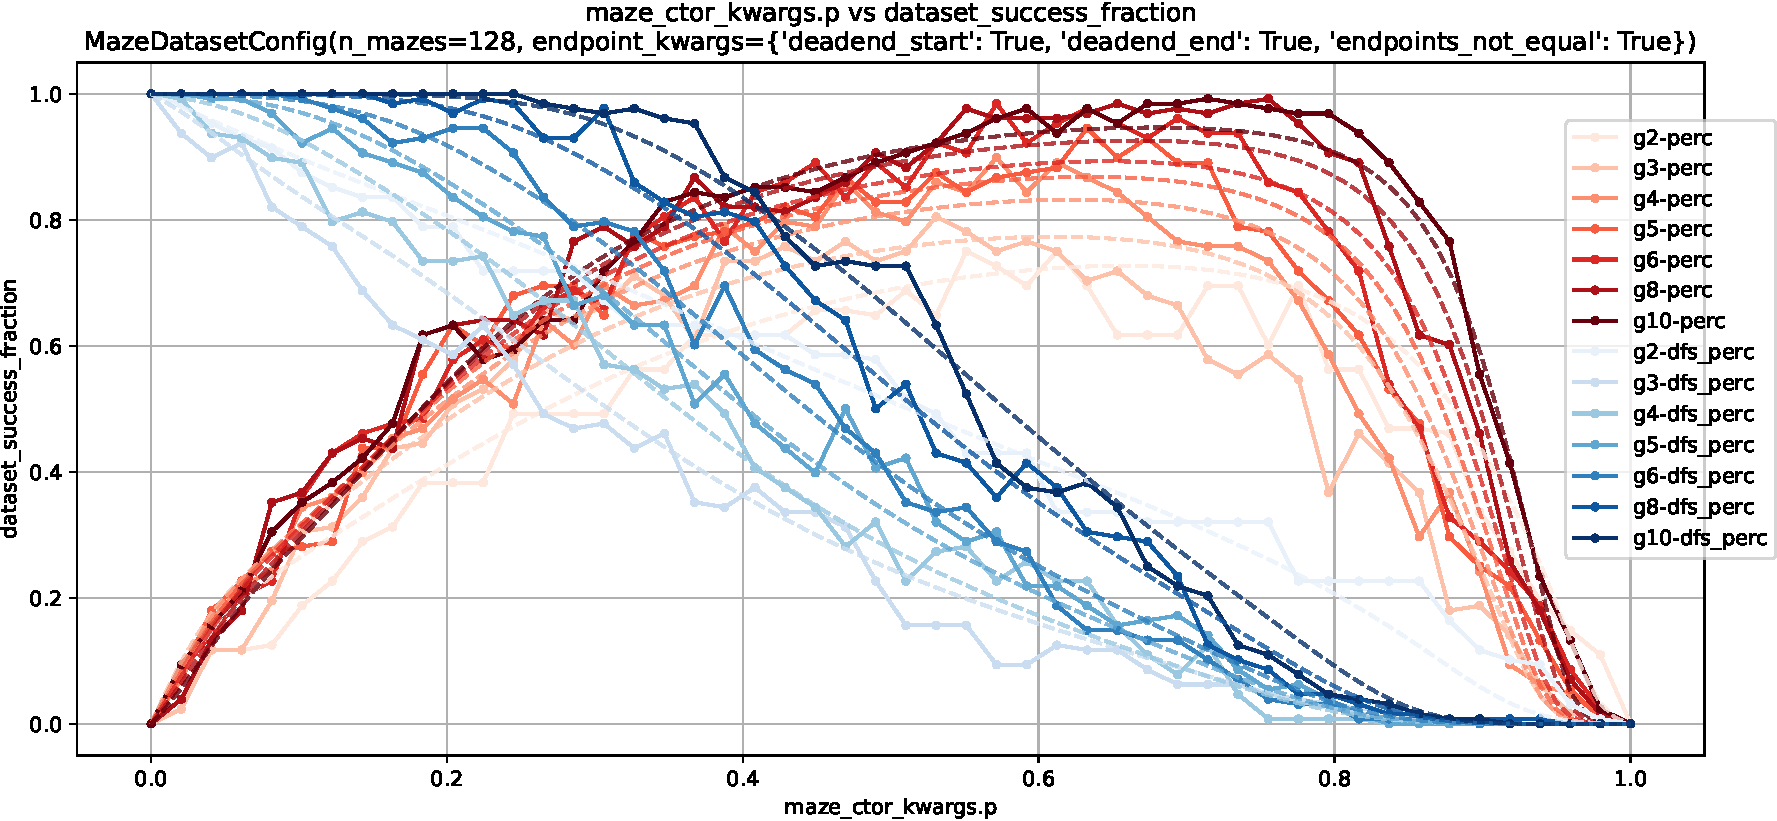
\includegraphics[width=1\textwidth,height=\textheight]{figures/ep/ep_deadends_unique-crop.pdf}
	\caption{
		In order to replicate the exact dataset distribution of \cite{easy_to_hard}, the parameter \href{https://understanding-search.github.io/maze-dataset/maze_dataset/dataset/maze_dataset_config.html#MazeDatasetConfig.endpoint_kwargs}{\texttt{MazeDatasetConfig.endpoint\_kwargs}} allows for additional constraints, such as enforcing that the start or end point be in a ``dead end'' with only one accessible neighbor cell. However, combining these constraints with cyclic mazes can lead to an absence of valid start and end points. To deal with this, our package provides a way to estimate the success rate of a given configuration using a symbolic regression model trained with PySR \cite{pysr}.
		An example of both empirical and predicted success rates as a function of the percolation probability \(p\) for various maze sizes, percolation with and without depth first search, and \texttt{endpoint\_kwargs} requiring that both the start and end be in unique dead ends. Empirical measures derived from a sample of 128 mazes. More information can be found on the \href{https://understanding-search.github.io/maze-dataset/benchmarks/}{benchmarks page} and in the notebook \href{https://understanding-search.github.io/maze-dataset/notebooks/estimate_dataset_fractions.html}{\texttt{estimate\_dataset\_fractions.ipynb}}.
	}
	\label{fig:sre}
\end{figure}